\chapter{High-Entropy alloys}
\label{sec:HEA}

High-Entropy Alloys (HEAs) has become an increasingly popular field in materials science, from to the large flexibility and possibilities for discovering new materials with unique properties. Since the original discovery in 2004, as of 2015 there has been over 1000 published journal articles on high-entropy alloys \cite{hea2016_ch1}. In the following section we will cover the fundamentals and some applications of high-entropy alloys. This section is be based on the fantastic description of HEAs in the book "High-Entropy Alloys - Fundamentals and Application", in particular chapters 1,2,3 and 7 \cite{hea2016_ch1}, \cite{hea2016_ch2}, \cite{hea2016_ch3}, \cite{hea2016_ch7}, and references therein.

\section{Fundamentals} 
A high entropy alloy can in a way be compared to a smoothie. In a smoothie one can produce unique combinations of flavors and nutritional values based on both the properties of the individual fruits and vegetables, and their interplay in the mixture. In materials science, a similar approach can be applied to generate a large range of materials with tunable properties depending on the intended application. In respect to HEAs, examples can be increased strength, ductility, corrosive resistance and low thermal conductivity. Moving on from the rather banal fruit analogy, a high-entropy alloy can be defined from two conditions:
\begin{enumerate}
    \item The material consists of at least 5 distinct elements, where each element contribute between 5-35$\%$ of the composition.
    \item The total configurational entropy is greater than 1.5R, where R is the gas constant. 
\end{enumerate}
The latter is an especial case for high-entropy alloys. The ideal configurational entropy of a random N-component solid-solution is described as
\begin{equation}
\Delta S_{\text{config}} = -R \sum_{i=1}^{N}X_i\ln X_i,
\end{equation}
where $X_i$ is the mole fraction of the $i$th component. Its clear that $\Delta S_{\text{config}}$ increase with a higher number of constituents in the mix. For instance, the ideal configurational entropy of a equimolar binary alloy is 0.69 R, as opposed to 1.61 R in a five-component equimolar alloy. If we neglect the other factors that influence the formation of solid solutions (will be covered later), from Gibbs free energy
\begin{equation}
\Delta G_{\text{mix}} = \Delta H_{\text{mix}} - T\Delta S_{\text{mix}},
\end{equation} 
the two primary factors in formation of solid solution is the mixing enthalpy, which is the driving force to form compounds, and the mixing entropy which is the driving force to form random solid solutions. At elevated temperatures especially, the energy associated to the entropy of the system becomes comparative to the mixing enthalpy and can impact the formation. In summary, the overall concept of high-entropy alloys is that through alloying a greater number of elements, the gain in configurational entropy of the system prohibits the formation of intermetallic compounds, in favor of random solid solution. The random term simply relate to the various components occupying lattice positions based on probability. In fact, a narrower definition of high-entropy alloys would be structures with a single-phase disordered solid solution. The two "definitions" given previously, can be considered as guidelines for the latter.
 
Although the mixing entropy mentioned above plays a central role in the formation, there are other factors to consider that can either favor or oppose the formation of a single disordered phase. One of these is the atomic size effect, which is related to the differences in atomic size between constituents in the alloy. This quantity is denoted $\delta$. Y. Zhang et al. in 2008 illustrated the relationship between $\Delta H_\text{mix}$ and $\delta$. When $\delta$ is very small, in other words when the alloys are comprised of elements with similar atomic sizes, the elements have an equal probability to occupy lattice sites to form solid solutions, but the mixing enthalpy is not negative enough to promote formation of solid solution. Increasing $\delta$ results in greater $\Delta H_\text{mix}$, but leads to a higher degree of ordering. The formation of solid solution high-entropy alloys occur in a narrow range of $\delta$ values, that satisfy both the enthalpy of mixing and the disordered state. Recently, Yang and Zhang proposed the parameter $\Omega$ to evaluate the stability of high-entropy alloys. This quantity is a product of the melting temperature $T_m$, mixing entropy and mixing enthalpy in the following relation

\begin{equation}
\Omega = \frac{T_\text{m} \delta S_\text{mix}}{|\Delta H_\text{mix}|}.
\end{equation}

They found that the formation of single disordered solid solution occurs at $\Omega \geq 1.1$ and $\delta \leq 6.6\%$, while compounds such as intermetallics form for greater values of $\delta$ and lesser values of $\Omega$. Similarly, replacing the atomic size effect with the number of elements results in an equivalent condition. These findings are summarized in figure 2.1.
\begin{figure}[H]
\centering
\begin{subfigure}{.85\textwidth}
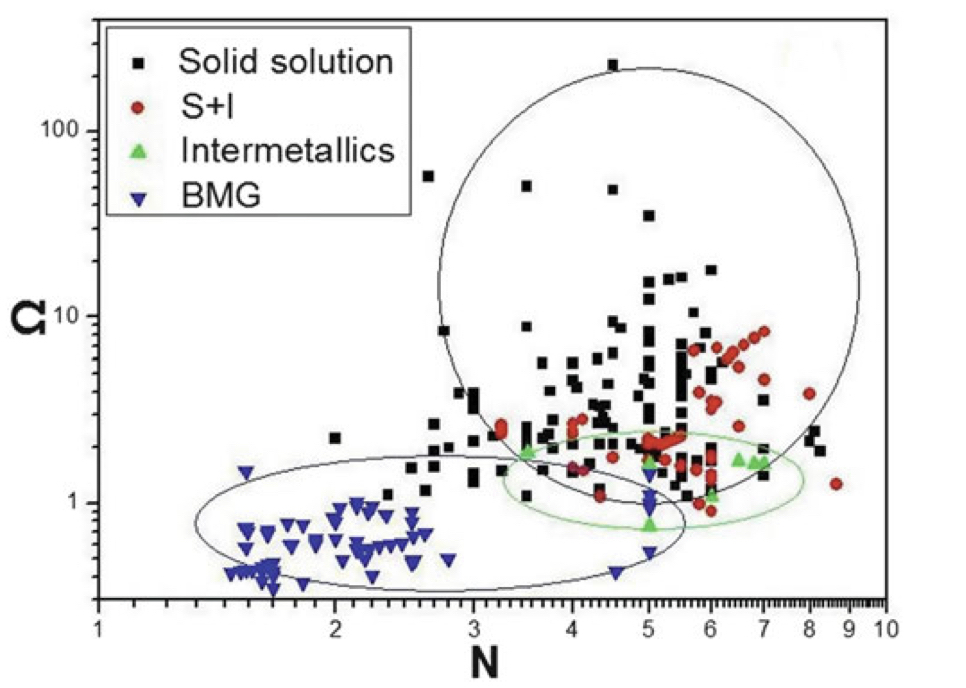
\includegraphics[width=\textwidth]{theory/heaformation1.jpeg}
\caption{HEA formation based on $\Omega$ and the atomic size effect $\delta$}
\end{subfigure}
\begin{subfigure}{.85\textwidth}
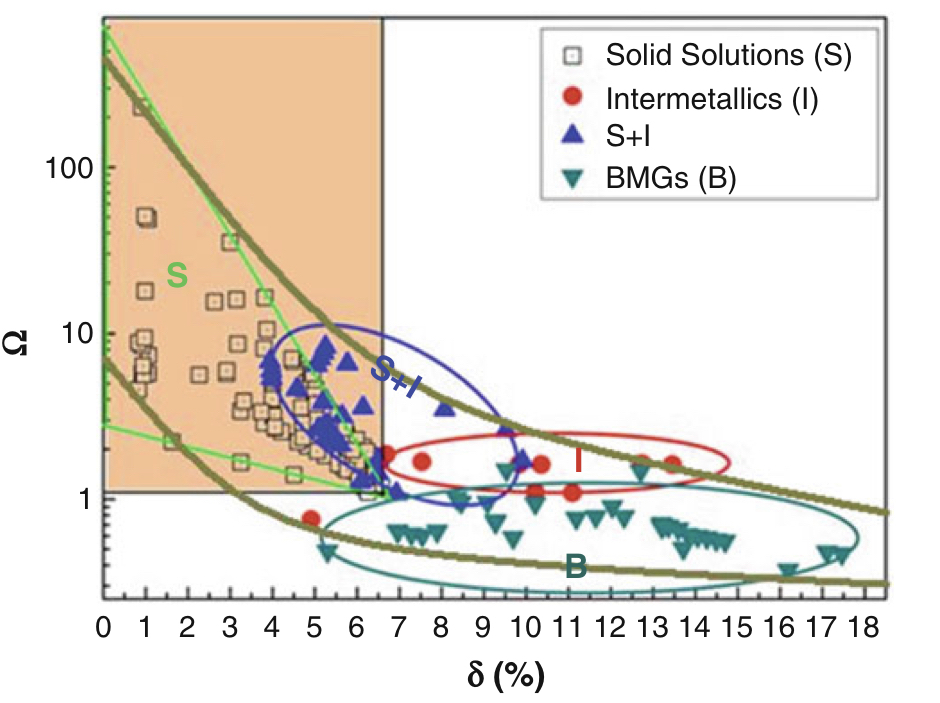
\includegraphics[width=\textwidth]{theory/heaformation2.jpeg}
\caption{HEA formation based on $\Omega$ and the number of consituents $N$}
\end{subfigure}
\caption{Formation of HEAs based on $\Omega = \frac{T_\text{m} \delta S_\text{mix}}{|\Delta H_\text{mix}|}.$, the atomic size effect $\delta$, and number of constituents $N$. Figures adopted from \cite{hea2016_ch2}}
\end{figure} 
An important quantity in terms of characterizing high-entropy alloys, is the total number of valence electrons VEC. Derived from the work of Guo et al. on the phase stability of the \ch{Al_xCrCuFeNi_2} HEA, the VEC can be directly related to the crystal structure of high-entropy alloys. A lower VEC stabilize the BCC phase, while higher values stabilize FCC, in between is a mixture of the two. Specifically values greater than 8.0 stabilize FCC, and values bellow 6.87 favor BCC. However, these boundaries are not rigid when including elements outside of transition metals, exceptions has also been found for high-entropy alloys consisting of manganese. Although a heavy majority of reported high-entropy alloys that form solid solutions has been found to adopt simple cubic structures, such as FCC and BCC. In addition to the high-entropy silicides mentioned in the introduction, recent studies has reported HEAs in less symmetric structures, such as \ch{CoFeMnTi_x V_y Zr_z}, \ch{CrFeNiTiVZr} and \ch{CoFeNiTi} in HCP, as well as the \ch{Ti_{35}Zr_{27.5}Hf_{27.5}Ta_5Nb_5} HEA in the orthorhombic crystal system.  

\section{Core effects and properties}
In this section, we will summarize the discussion above into four core effects that can be used to explain high entropy alloys, and discuss some of the properties observed in various HEAs. The first core effect is called the "high-entropy effect", as explained in the previous section the high configurational entropy of HEAs compared to traditional solids or even binary alloys is central to stabilize the disordered phase ahead of intermetalic or strongly ordered structures. This effect can result in enhanced strength and ductility. From considerations of Gibbs free energy, we see that this effect is most prominent at elevated temperatures.

The second effect is the "severe lattice distortion effect" that arises from the fact that every element in a high-entropy structure is surrounded by non-homogeneous elements, thus leading to severe lattice strain and stress. The overall lattice distortion is additionally attributed to the differences in atomic size, bonding energies and crystal structure tendencies between the components. Therefore, the total lattice distortion observed in HEAs are significantly greater than that of conventional alloys. This effect mostly affects the strength and conductivity of the material, such that a higher degree of distortion yields greater strength and greatly reduces the electronic and thermal conductivity due to increased electron and phonon scattering. An upside to this is that the scattering and following properties become less temperature dependent given that it originates from the lattice rather than thermal vibrations. The concept of lattice strain in high-entropy alloys can be visualized as in figure 2.2 below. 

\begin{figure} 
\centering
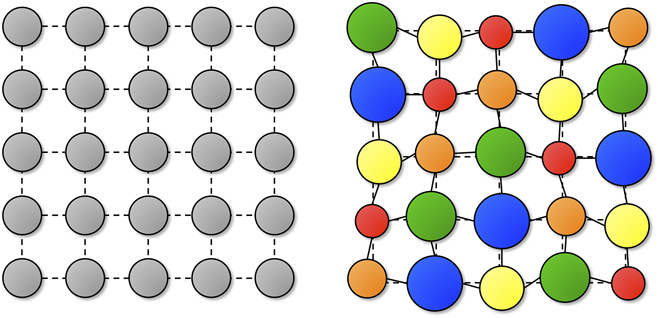
\includegraphics[width=\textwidth]{theory/latticeDistortionHEA.jpeg}
\caption{A schematic illustration of lattice distortion in high-entropy alloys, compared to conventional materials. Figure from \cite{owen_jones_2018}.}
\end{figure}
 
The two remaining effects, "sluggish diffusion" and "cocktail effect" can be summarized swiftly. The first is a direct consequence of the multi-component layout of high-entropy alloys that results in slowed diffusion and phase transformation because of the number of different elements that is involved in the process. The most notable product from this effect is an increased creep resistance. Lastly, we have the cocktail effect which is identical to the smoothie analogy mentioned previously, in that the resultant characteristics of a high-entropy alloy is a combination of both the individual elements and their interplay. This is possible the most promising concept behind high-entropy alloys, which fuels researchers with ambitions to discover highly optimized materials by meticulously combining and predicting properties from different elements. Examples of this can be the refractory HEAs developed by the "Air Force Research Laboratory" that significantly exceeded the melting points and strength of previous Ni or Co-based superalloys, by alloying specifically refractory elements such as Mo. Nb and W. Another example is the research conducted by Zhang et al. on the high-entropy system \ch{FeCoNi(AlSi_x)}, with ($0 < x 0.8$). In this HEA it was found that increased amount of either Al or Si lowered the saturation magnetization of the alloy. By tuning the relative amounts, it was found excellent properties for an $x=0.2$ HEA in terms of the magnetization, electrical resistivity and yield strength to produce a promising soft-magnet. The same was also found in \ch{Al_{0-2}CoCrFeNi} HEAS, where the addition of Al reduced the ferromagnetism of the alloy, and in \ch{CoCrCuFeNiTi_x} alloys where $x = 0$ was paramagnetic and $x > 0.8$ showed superparamagnetic properties. In general we find that that the saturation magnetism is mostly dependent on the contents and distribution of ferromagnetic elements such as Fe, Co and Ni while the addition of anti-ferromagnets like Cr could be difficult to predict. For example in the ferromagnetic HEA CoFeMnNiX, X = Al, Cr, Ga, Sn, studied in \cite{ZUO201710}, Mn pushed the material to the ferromagnetic phase, meanwhile addition of Cr pushed the material to a paramagnetic phase. Likewise in the equimolar system of \ch{CrMnFeCoNi} \cite{PhysRevB.96.014437}, the local magnetic moment of Cr was found to align antiferromagnetic, and the ferromagnetic character was attributed to local magnetic moments around Fe and Mn. 

As we have seen from the above examples, what makes high-entropy alloys a particularly interesting and promising field, is that they possesses the ability to be tuned for specific applications and properties, by testing specific combinations and distributions of different elements. In many ways, not indifferent to a smoothie or a cocktail.